\chapter{针对移动相机的实时视频背景减除技术}
\label{ch5:RMCBS}

在本文第~\ref{ch4:FMCBS}章中提出了一种针对移动相机拍摄视频的快速背景减除算法,该算法能以8帧/秒的速度处理分辨率为$640 \times 480$的视频,而且前景检测准确度达到与当前先进算法接近的水平。虽然第~\ref{ch4:FMCBS}章中提出的快速算法的速度已经比当前领先的一些算法\cite{gbsuperpixel}快几十倍,但是距离实时处理还有一段距离。在一些应用场景下, 如实时监控以及海量监控视频中的移动目标搜索等, 背景减除算法的速度比准确度更重要, 而目前还没有一种算法能实现实时地提取移动相机拍摄视频中较为准确的前景。本章针对实时视频背景减除应用需求,重点研究了实时视频背景减除算法的实现,提出一种简单有效的实时算法。假设视频中大部分区域是背景, 前景只占相对较小部分。 在大多数情况下, 在现实场景中拍摄的视频几乎都满足这个假设。在预处理阶段,首先用基于超像素的区域增长预处理算法得到可能是前景的超像素; 然后基于分块相对光流的背景特征点筛选算法来估算相机运动; 最后检查光流与相机运动的一致性, 得到背景减除的最终结果。 实验结果表明, 该算法可以实时处理大小为$640 \times 480$像素的视频, 且前景检测准确度优于同类实时算法。



\section{相关工作}
\label{ch5:sec:relatedWorks}
 文献~\inlinecite{5.8s}提出一种实时的移动相机下视频背景减除算法。 该算法利用双模式单高斯模型对背景进行建模。使用双模式的高斯模型一方面可以防止前景像素对背景模型产生 干扰,影响背景模型的准确度;另一方面也可以使得背景模型能够适应背景部分像素的变化。此外为了处理相机运动情况,在高斯模型中加入了模型生存时间变量(age)来动态自适应地调整模型更新率。为了加快速度,文献~\inlinecite{5.8s}将输入图像平均分为$ N \times N $ 个均匀网格,每个网格内用一个高斯模型进行背景建模。假设$t$时刻位于网格$i$内的像素集合为$ G_{i}^{(t)}$,网格$i$内的像素个数为$ |G_{i}^{(t)}|$,当观察到像素$ I_j^{(t)}$时,$G_i^{(t)}$内的高斯模型的均值$ \mu_i^{(t)}$,方差$ \sigma_i^{(t)}$ 以及模型生存时间$\alpha_i^{(t)}$ 的更新策略为:
 $$\mu_i^{(t)} = \frac{\hat{\alpha_i^{(t-1)}}}{\hat{\alpha_i^{t-1}}+1}\hat{\mu_i^{(t-1)}} + \frac{1}{\hat{\alpha_i^{(t-1)}}}M_i^{(t-1)}$$

$$\sigma_i^{(t)} = \frac{\hat{\alpha_i^{(t-1)}}}{\hat{\alpha_i^{t-1}}+1}\hat{\sigma_i^{(t-1)}} + \frac{1}{\hat{\alpha_i^{(t-1)}}}V_i^{(t-1)}$$

$$ \alpha_i^{(t) = \hat{\alpha_i^{(t-1)}}}+1$$
其中 $M_i^{(t-1)}$,$V_i^{(t-1)}$分别定义为:
$$ M_i^{(t)} = \frac{1}{|G_i|}\sum_{j\in G_i}I_j^{(t)}$$
$$ V_i^{(t)} = \max_{j \in G_i}{(\mu_i^{(i)})-\mu_j^{(t)}}^2 $$
在文献~\inlinecite{5.8s}算法中,每个网格内同时维护两个高斯模型,其中一个为当前起作用的模型$Model_a$,另一个为候选模型$Model_c$。当观察到当前帧图像与$Model_a$匹配时,利用上述的更新策略对$Model_a$进行更新;若当前帧图像与$Model_c$匹配时,利用同样的更新策略对$Model_c$进行更新。在模型匹配计算前景对象时起作用的一直是$Model_c$,当$Model_c$的生存时间大于$Model_s$的生存时间时,将其两者交换。这种双模式的单高斯模型在效率上比混合高斯模型(GMM)效率更高,且能处理包含动态背景的视频。由于相机是运动的,每次在匹配模型时需要估算相机的运动并进行补偿,返回到静态相机情形。文献~\inlinecite{5.8s}算法利用每个网格点的KLT~\cite{KLT}跟踪结果估算单应性矩阵的方式实现。在相机运动补偿后,根据基于像素点和网格中心点的距离的权值,利用周围多个网格高斯模型加权得到像素点位置的高斯模型,通过模型匹配得到像素前景分割结果。由于模型简单,文献~\inlinecite{5.8s}的速度非常快,甚至能在智能手机上实现实时检测。但是文献~\inlinecite{5.8s}没有给出该算法前景检测准确度的定量分析,且实验所用的视频均较容易识别前景。通过实验,作者发现在常用数据库视频的测试中,文献~\inlinecite{5.8s}算法的前景检测准确度较低,而且无法处理相机快速移动的情况。\par

文献~\cite{ACPRRealTime}提出了一种基于像素点轨迹的准实时移动相机视频前景提取算法。该算法处理分辨率为$640 \times 480$的视频的速度约为1.8帧/秒。在针对移动相机的视频背景减除算法中,基于像素点轨迹的方法是主要类型之一。假设在视频中的$F$帧图像中一共有$P$个像素点轨迹,第$i$个像素点的轨迹可以表示为$w_i={[x_{1i}^T \cdots x_{Fi}^{T}]}^T \in \mathbf{R}^{1 \times 2F}$,其中在每一帧图像中像素点的坐标为$ x_{fi} = {[u_{fi},v_{fi}]}^T$。所有这些像素点轨迹组成了一个$2F \times P$的矩阵:
\begin{equation}
\label{ch5:equ:trajmatrix}
\mathbf{W}_{2F \times P} = {[w_{1}^T \cdots w_{P}^T]}^T = \begin{Bmatrix}
u_{11} & \cdots & u_{1P} \\
v_{11} & \cdots  &  v_{1P}\\
 \vdots &  & \vdots \\
 u_{F1}& \cdots & u_{FP}\\
 v_{F1}& \cdots & v_{FP}
\end{Bmatrix}
\end{equation} \par

假设相机成像时满足正交投影,在理想情况下,公式~\ref{ch5:equ:trajmatrix}中的$\mathbf{W}$矩阵的秩应该为3\cite{Tomasi_1992}。由于通过特征点跟踪获取像素点的长期轨迹非常耗时,文献~\cite{ACPRRealTime}提出只利用前一帧图像来获取像素点轨迹,即每个轨迹通过两个特征点的位置之差来计算,第$i$个特征点可以用二维空间向量$\mathbf{v_i}=(dx_i,dy_i) \in \mathbf{R}^2$表示。此外该算法中还利用基于分块的方法获取稀疏的轨迹集合,将图像分为$N \times N$个分块,像素点轨迹矩阵为:
$$ \mathbf{W}_{2 \times (N \times N )} = {[v_{1}^T \cdots v_{N \times N}^T]}^T = \begin{Bmatrix}
dx_1 & \cdots & dx_{N \times N} \\
dy_1 & \cdots & dy_{N \times N}
\end{Bmatrix}$$
利用简化后的矩阵,文献~\cite{ACPRRealTime}算法对轨迹点进行聚类将轨迹点分为背景轨迹点和前景轨迹点两类,最后将轨迹点的标记信息扩散到整幅图像获取每个像素点的前景/背景标记。文献~\cite{ACPRRealTime}的算法在Hopkins数据集中的视频上\cite{HopKinsDataSet}得到的F-Score大约在0.7左右,比文献~\cite{5.8s}算法的准确度高,但是其速度只有不到2帧/秒,远没有达到实时处理的速度。\par

Wang等人~\cite{WangTMM2014}提出了一种多个视频的共同前景提取算法,从一组视频中提取其中共有的前景对象。该算法利用时间连续的超像素算法(temporal superpixels, TSP )对视频中连续的视频帧图像进行分割,将不同视频中的共有前景对象归为同一类。本章提出的算法在流程上与文献~\inlinecite{WangTMM2014}中的算法有相似之处,均是先对视频图像帧进行超像素分割, 然后对超像素进行合并得到前景线索,不同之处是文献~\inlinecite{WangTMM2014}处理的是提取多个视频中的共同前景问题, 且本章算法所采用的单图像超像素分割算法以及区域合并算法均与文献~\inlinecite{WangTMM2014}有较大区别。 此外,文献~\inlinecite{WangTMM2014}还提出了一种基于MRF的优化过程对结果进行求精, 能准确地提取多个视频中共同的前景,主要用于视频编辑等领域。




\section{算法描述}
\label{ch5:sec:algorithm}
本文算法的流程如图~\ref{ch5:fig:flowchart}所示。首先对图像进行超像素分割,考虑背景像素的连续性, 提出一种基于超像素的区域增长算法对图像进行图像分割预处理。利用背景部分连续性特点,以区域合并的方式不断扩大背景区域的范围。预处理过程结束后得到一个图像区域分割结果,其中大部分背景像素集中在大区域中,属于前景的对象和一些包含边缘和角点的前景处在面积较小的区域中。因此对这部分可能是前景的小区域再进行进一步计算。 为了估算相机运动, 提出一种基于相对光流的特征点筛选算法,筛选出属于背景的特征点, 并利用这些特征点以分块的方式估算相机的运动。 最后通过比较这些超像素的光流与所估算的相机运动的一致性来确定最终的前景。 本文算法简单直接, 不需要建立任何背景模型和计算点轨迹,利用GPU和CPU的混合编程可以实现实时处理。 大量实验证明, 本文算法的前景检测准确度F-Score值达到了0.75左右,高于同类实时算法\cite{5.8s}。下面对各主要部分进行详细描述。
\begin{figure}
  \centering
  % Requires \usepackage{graphicx}
  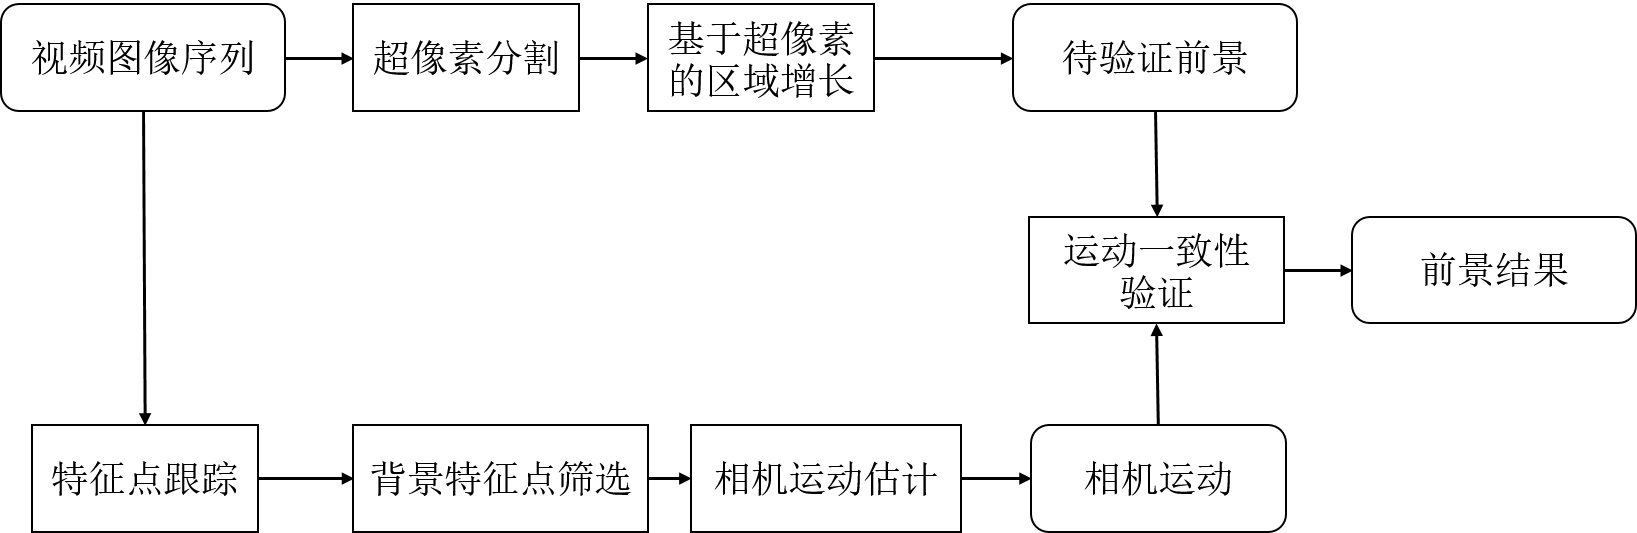
\includegraphics[width=0.7\textwidth]{ch5/fig1.png}\\
  \caption{算法流程图}\label{ch5:fig:flowchart}
\end{figure}

\subsection{基于超像素的区域增长算法}
对于自然场景中所拍摄的视频,其背景和前景的一个显著区别是背景通常具有连续性,如天空、树、 墙面、地面等。 这些部分像素的特点是在周围较大的区域内存在与其相似的像素。
 如图~\ref{ch5:fig:cont}所示,图~\ref{ch5:fig:sub:img}是视频中的一帧图像, 图~\ref{ch5:fig:sub:imgCont}中用不同颜色标注不同背景区域(绿色表示树林区域,灰色表示地面区域)。人眼在观察图~\ref{ch5:fig:sub:img} 时,很快能发现图像中背景部分包括树林和地面等, 这些部分的像素具有明显的连续性; 相反, 作为前景的汽车上的像素则没有这种连续性。\par

 \begin{figure}[htb]
  \centering%
  \subcaptionbox{输入图像\label{ch5:fig:sub:img}} %标题的长度,超过则会换行,如下一个小图。
    {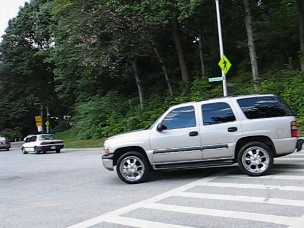
\includegraphics[width=0.4\textwidth]{ch5/fig2a.png}}%
 \hspace{1em}%
  \subcaptionbox{连续性区域\label{ch5:fig:sub:imgCont}}
      {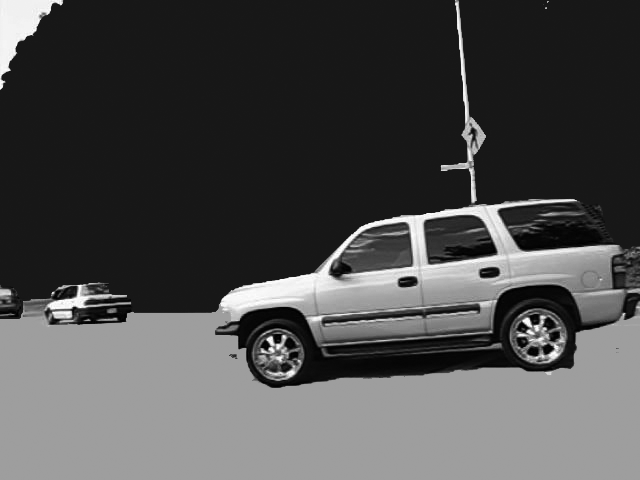
\includegraphics[width=0.4\textwidth]{ch5/fig2b.png}}

  \caption{图像背景连续性示意图}\label{ch5:fig:cont}
\end{figure}
 针对这种特点,受到基于区域增长的图像分割算法~\cite{seededRegionGrowing}的启发, 本章提出一种基于超像素的区域增长算法对待处理图像进行预处理,得到具有连续性的背景部分。 为了提高效率,首先对图像进行超像素分割~\cite{superpixel}. 采用基于颜色直方图和梯度直方图距离的方式来比较超像素区域之间的相似性
\begin{equation}\label{ch5:equ:distance}
S_d(x,y) = c \times D_c(x,y) + (1-c) \times D_g(x,y)
\end{equation}

其中, $D_c(x,y)$是区域之间的颜色直方图的距离,$D_g(x,y)$表示梯度直方图的距离。 本章算法在RGB色彩空间建立包含4096个单元的直方图来描述超像素的颜色特征, 另外利用36个单元的梯度直方图来表示超像素的梯度特征。 采用巴氏距离来计算直方图之间的距离,具体公式见~\ref{subsec:mergeP1}节。式~\ref{ch5:equ:distance}中, $c$是加权系数, 其值可以通过超像素之间的平均距离来确定,$c = D_c / (D_c + D_g)$  , 其中$D_c$,$D_g$分别表示图像中相邻超像素之间颜色直方图和梯度直方图的平均距离。与~\ref{ch4:sec:sub:ssrg}节中的~\ref{ch4:alg:ssrg}算法类似,本章提出了一种基于超像素的区域增长预处理方法,见算法~\ref{ch5:alg:srg},对视频图像帧进行预处理,获得可能的前景区域的线索。本章预处理算法与~\ref{ch4:alg:ssrg}算法不同之处在于~\ref{ch4:alg:ssrg}算法利用图像的连续性特点将已知的背景种子点扩展到整幅图像,将图像分为前景和背景两个区域;而本章提出的~\ref{ch5:alg:srg}算法通过随机选取种子点的方式,以贪心算法的方式通过区域增长将图像分为多个区域,其中面积大的区域因为具有较强的连续性,是背景的概率较大;而面积较小的区域为前景的几率较大。
\renewcommand{\algorithmcfname}{算法}
\begin{algorithm}[ht]
\caption{基于超像素的区域增长算法}
\label{ch5:alg:srg}
\LinesNumbered
\KwData {图像$I$的超像素$S$, 超像素区域增长门限$T$ }
\KwResult {区域分割结果$R$}
  $i=0$, 初始化空集$C$ \;
 随机选择一个超像素$s$作为种子点\;
 将$s$添加到$C$ \;
 \While {$C$不为空}{
 从$C$中取一个超像素$s$, 将其加入区域$R[i]$ \;
 $i++, D=0,$ 初始化空集$N$ \;
 \While {$D<T$} {
 将$s$四邻域中未访问的超像素加入$N$ \;
  $S_m = \arg \min_{s \in N}S_d(s,R[i])$ \;
 $D=S_d(S_m,R[i])$\;
 $S_m$加入$R[i]$, $s=S_m $\;
 更新$R[i]$直方图\;
 从$N$中删除$S_m$\;}
 将$N$中的超像素添加到$C$中\;}
\end{algorithm}

算法~\ref{ch5:alg:srg}中,$T$的值为$T= c \times D_c + (1-c) \times D_g$。图~\ref{ch5:fig:srg}所示为区域增长算法的一个计算实例。 图~\ref{ch5:fig:sub:superpixel}是输入图像的超像素分割结果, 图~\ref{ch5:fig:sub:srg}是区域增长算法的输出结果, 其中用不同的颜色表示不同的区域。 从图~\ref{ch5:fig:sub:srg}中可以看到, 算法~\ref{ch5:alg:srg}能有效地将具有连续性的背景区域超像素合并到一起, 使得这些大区域所包含的超像素数量要明显多于前景区域。 因此本章算法直接将预处理后超像素数量大于15的区域所包含的超像素判为背景。 对于剩下的超像素, 再用~\ref{ch5:sec:sub:sub:motionC}节介绍的算法, 根据其光流与相机运动的一致性来进一步判断其是否为前景。
 \begin{figure}[htb]
  \centering%
  \subcaptionbox{超像素分割结果\label{ch5:fig:sub:superpixel}} %标题的长度,超过则会换行,如下一个小图。
    {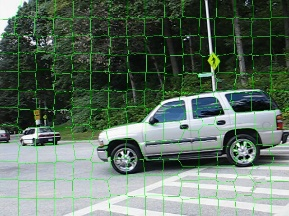
\includegraphics[width=0.4\textwidth]{ch5/fig3a.png}}%
 \hspace{1em}%
  \subcaptionbox{区域增长结果\label{ch5:fig:sub:srg}}
      {
\includegraphics[width=0.4\textwidth]{ch5/fig3b.png}}

  \caption{图像背景连续性示意图}\label{ch5:fig:srg}
\end{figure}

\subsection{运动一致性验证}
\label{ch5:sec:sub:motionv}

\subsubsection{特征点筛选}
\label{ch5:sec:sub:sub:fp}
 为了估算相机运动,首先通过KLT算法~\cite{KLT}对相邻帧进行特征点提取和匹配。得到匹配特征点后,需要筛选出属于背景特征点, 并用它们来估算描述相机运动。在文献~\inlinecite{5.8s} 中, 基于相机运动可以用一个全局单应性矩阵描述这一假设,使用RANSAC 算法来筛选背景特征点。实际上, 根据多视图几何原理,在相机自由运动的情况下这一假设并不一定成立~\cite{Multitransform}。 假设在世界坐标系下, 三维空间场景点用齐次坐标$\mathbf{X}={(x,y,z,w)}^T$表示, $\mathbf{p}$ 为其投影到二维图像中的坐标。其投影关系为$\mathbf{p} = \mathbf{QX} = \mathbf{K[I|0]X}$ ; 其中, $\mathbf{K}$ 是摄像机参数矩阵, $\mathbf{Q}$ 是一个3 行4 列的矩阵。 当摄像机有旋转$\mathbf{R}$ 和平移$\mathbf{T}$时, $\mathbf{X}$将投影到另一帧图像,其坐标为 $\mathbf{\acute{p}}=\mathbf{\acute{K}[R|T]X}$, 这时$\mathbf{p}$ 与$\mathbf{\acute{p}}$ 之间并不存在一对一的映射关系。 考虑以下2 种特殊情况:
 \begin{enumerate}
   \item 若摄像机没有平移只有旋转, 有$\mathbf{\acute{p}}=\mathbf{\acute{K}RX}$, 即$\mathbf{p}$ 与$\mathbf{\acute{p}}$ 之间的变换可以用单应性矩阵$\mathbf{H}_R$表示。
   \item 若场景点共面, 不失一般性, 假设场景点都位于平面$z=0$之上。 矩阵$\mathbf{Q}$的第3列可以忽略, 因此有:


    $$\mathbf{p}=[\mathbf{Q_1},\mathbf{Q_2},\mathbf{Q_4}]\mathbf{X} = \mathbf{HX},  \mathbf{\acute{p}}=[\mathbf{\acute{Q}_1},\mathbf{\acute{Q}_2},\mathbf{\acute{Q}_4}]\mathbf{X} = \mathbf{\acute{H}X},  $$
   $$ \mathbf{\acute{p}} = (\mathbf{\acute{H}\acute{H}^{-1}})=\mathbf{H}_{\pi} \mathbf{p} $$


  即$\mathbf{p}$ 与$\mathbf{\acute{p}}$ 之间的变换可以用单应性矩阵$\mathbf{H}_{\pi}$表示。
 \end{enumerate}


当相机运动不满足上述2个假设时, 不能用一个全局单应性矩阵来描述相机运动。由于RANSAC算法只能用于估算单一模型, 在这种情况下用RANSAC算法筛选出的背景特征点时可能会有较大误差。考虑到无论相机如何运动, 前景相对于背景都是运动的,可以利用这种相对的运动区分前景特征点和背景特征点。 假设视频中相邻图像帧$I_1,I_2$ 的匹配特征点分别为$\mathbf{p}$ 和$\mathbf{\acute{p}}$, 若已知$I_1$中的某个特征点$\mathbf{A}$是属于背景的特征点,那么在理想情况下,$I_1$中的其他的背景特征点$\mathbf{p}_b$与$\mathbf{A}$应该是相对静止的; 在$I_1$中 $\mathbf{p}_b$与$\mathbf{A}$ 对应的特征点分别用$\mathbf{\acute{p}}_b$ 和$\mathbf{\acute{A}}$ 表示,这种相对静止的关系可以表示为:
\begin{equation}
\label{ch5:equ:relFlow}
\begin{cases}
  \mathbf{V}_b = \mathbf{p}_b - \mathbf{A}  \\
   \mathbf{\acute{V}}_b = \mathbf{\acute{p}}_b - \mathbf{\acute{A}} \\
{\|\mathbf{V}_b-\mathbf{\acute{V}}_b\|}^2 < t
\end{cases}
\end{equation}
	 	
而对于前景特征点,因为其相对于背景发生了运动,其相对光流 并不满足公式\ref{ch5:equ:relFlow}; 其中,$ \mathbf{V}_f = \mathbf{p}_f - \mathbf{A},\mathbf{V}_f = \mathbf{\acute{p}}_f - \mathbf{\acute{A}}$  。\par
若考虑深度等因素对特征点位置的影响, 可能会有一些背景上的特征点并不满足公式\ref{ch5:equ:relFlow}。 而当$t$取值较小时, 几乎全部前景上的特征点都不会满足公式~\ref{ch5:equ:relFlow}。 在估算单应性矩阵时只需要最少4组特征点,因此在筛选时并不需要得到全部背景特征点, 只需去除位于前景上的特征点。 本文利用这种基于相对光流的思想,选取满足公式~\ref{ch5:equ:relFlow}的部分背景特征点来估算相机运动。实验中, 将$t$的值固定设置为1.0。 背景点$A$的选择算法为$A = \arg \min_{a}\sum_{p}{\|\mathbf{V}_{pa} - \mathbf{V}_{\acute{p}\acute{a}}\|}^2$ ,其中,$ \mathbf{V}_{pa} = \mathbf{p} - \mathbf{a}$。 为验证筛选算法的有效性, 定义误检率$P_e$为$p_b$中前景特征点所占百分比,$$P_e= \frac{|p_b \in F |}{|P_b|} \times 100. $$
作者在Hopkins视频数据库~\cite{HopKinsDataSet}中的10个视频上进行了实验, 对本章提出的背景特征点筛选算法与基于RANSAC的背景特征点筛选算法进行了对比。 实验中, 在所有视频中均将2种算法的阈值固定设为1.0。 本文算法得到的$P_e$平均值为$0.32 \%$, 而RANSAC算法筛选的背景特征点$P_e$平均值为$0.36\%$。 \par
本文提出的特征点算法的一个计算实例如图~\ref{ch5:fig:fpFilter}所示, 其中,红色圆圈标注的为筛选后得到的背景特征点, 蓝色圆圈标注的则为前景特征点,蓝色线连接的为背景点$A$和$\acute{A}$。\par
\begin{figure}[htb]
  \centering
  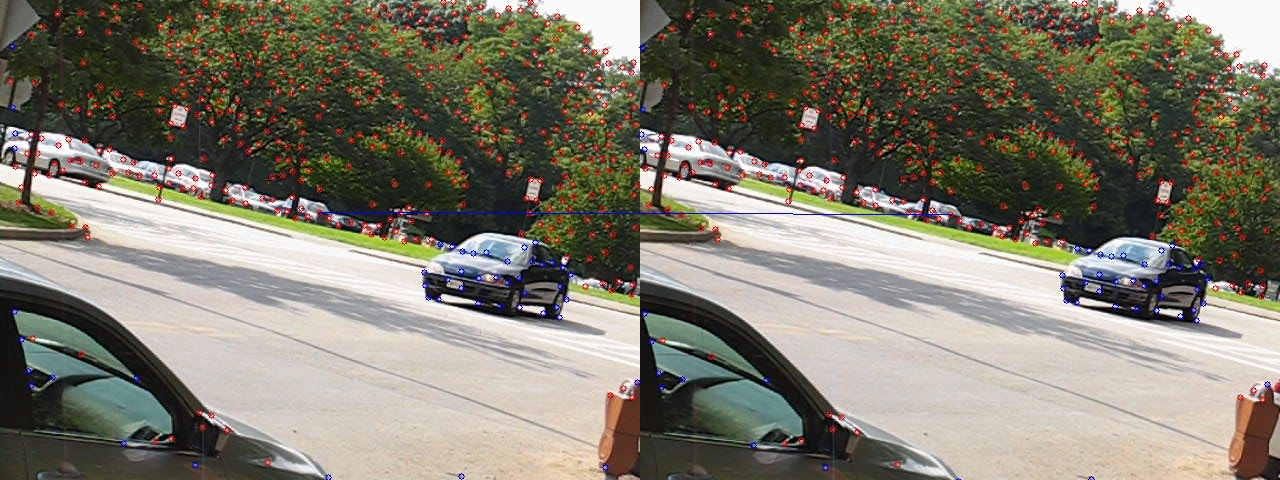
\includegraphics[width=0.95\textwidth]{ch5/fig4.png}
  \caption{基于相对光流的特征点筛选}\label{ch5:fig:fpFilter}
\end{figure}


\subsubsection{基于分块的单应性矩阵估算}
\label{ch5:sec:sub:sub:homography}
为了统一处理各种相机运动,本章提出一种基于分块的单应性矩阵估算算法, 使得图像中不同区域有不同的单应性矩阵。首先将视频帧图像均匀分为$N \times N $个均匀网格,分别在各个网格内估算适用于网格范围内的单应性矩阵用于描述区域内的运动情况。考虑到分块的连续性, 在计算某分块$A$的单应性矩阵时, 除了利用分块内的特征点, 还加入了其周围八邻域中已知单应性矩阵的分块$N$与$A$的边界点$p_B$。$p_B$为$N$和$A$中心点之间连线的中点。本章提出的基于分块的相机运动估算算法如算法~\ref{ch5:alg:blockHomo}所示。\par
\renewcommand{\algorithmcfname}{算法}
\begin{algorithm}[ht]
\caption{基于分块的相机运动估算算法}
\label{ch5:alg:blockHomo}
\LinesNumbered
\KwData {图像$I_{1},I_{2}$的匹配特征点对$F$, 网格大小$N$, 单应性矩阵估算最小特征点数 $F_{Min}$ }
\KwResult {单应性矩阵数组$H$}
 将$I_{1},I_{2}$均匀划分为$N \times N$个网格$cells$\;
\For {$i \leftarrow 1$ \KwTo $N \times N$}{
\If {$H[cells[i]]$已知}{
    继续循环\;}
     $F_i \leftarrow cells[i]$ 内的特征点对\;
    \ForEach{$cells[n] \in cell[i]$的八邻域}{
        \If {$H[cells[n]]$ 已知}{
        $B(i,n) \leftarrow (Center[cells[i]] +Center[cells[n])/2$\;
            将 $(B(i,n), H[cells[n]] \times B(i,n))$加入 $F_i$ \;
        }
    }
    $R \leftarrow 0$ \;
    \While{以$cells[i]$为中心半径为$R$区域${Set_{i,R}}$内的特征点$F_{i,R}$总数小于$F_{Min}$}{
        {$ R \leftarrow R+1$} \;
    }
    {利用$F_{i,R}$中的特征点对估算$h$ \;}
    \ForEach {$ cell \in {Set_{i,R}}$}
        {$H[cell] \leftarrow h$\;}
    }
\end{algorithm}


在齐次坐标下, $3 \times 3$的单应性矩阵有8个未知参数, 因此最少只需要4对匹配特征点就可以估算出矩阵。为了消除错误匹配特征点带来的误差, 将估算单应性矩阵的最小特征点数设为10。 本章算法假设在图像中背景区域的特征点数要大于这个最小门限, 在绝大部分视频中这个假设很容易满足。


\subsubsection{运动一致性验证}
\label{ch5:sec:sub:sub:motionC}

 对预处理后可能为前景的超像素, 利用KLT~\cite{KLT}计算超像素中心点的光流,并将其与估算的相机运动进行比较。假设像素点$\mathbf{p}=(x,y,1)$ 位于第$i$ 个分块内, 利用算法~\ref{ch5:alg:blockHomo} 得到的单应性矩阵数组$\mathbf{H}$ 可以得到变换后的坐标:
 $$ \mathbf{\acute{p}}_h = \mathbf{H}[i]p^T = {(w_x,w_y,1)}^T ,$$
设$\mathbf{p}$ 点的光流为$\acute{p}_f = (d_x,d_y)$ 。 通过超像素中心点处光流与相机运动的欧几里德距离$ D_{x,y} = \sqrt{{(w_x-d_x-x)}^2 + {(w_y - d_y -y)}^2}$  来度量这两者的一致性。当$ D_{x,y} > T_{fg}$时, 将该超像素判为前景,反之为背景。 其中$T_{fg}$ 固定设为2.0。

\section{实验结果与分析}
\label{ch5:sec:results}
 通过GPU和CPU的混合编程, 使用C++语言,借助CUDA~\cite{CUDA}和OpenCV~\cite{opencv_library}实现了本文的算法。 其中, 在GPU 上实现了文献~\cite{superpixel}中的超像素分割算法,利用OpenCV提供的GPU实现完成KLT~\cite{KLT}特征点跟踪。 实验中计算机配置为Intel i7 3.5 GHz CPU, NVIDIA GeForce Titan GPU。 为了测试算法的有效性, 在Hopkins视频数据库~\cite{HopKinsDataSet}中测试了本文算法。 该数据库中的视频包含各种复杂相机运动,是移动相机背景减除研究中较为常用的测试数据集。在实验中, 超像素大小约为1600像素, 在估算相机运动时将图像平均分为$8 \times 8$ 共64个单元的网格, 本文对所有测试视频保持同样的参数。
 为了便于观察算法的性能,在图~\ref{ch5:fig:MosegResults}中给出了部分随时间变化的多帧图像的背景减除结果。其中,(a)-(d)中分别为Cars2、Cars6、People1和People2视频中的第2、10、15、20、25帧图像得到的背景减除结果。\par
 \begin{figure}[htb]
\begin{center}
 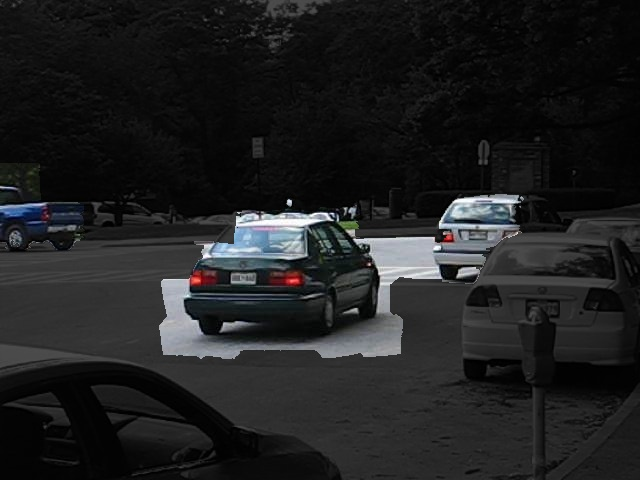
\includegraphics[width=0.18\textwidth]{ch5/moseg/c2_02.jpg}
  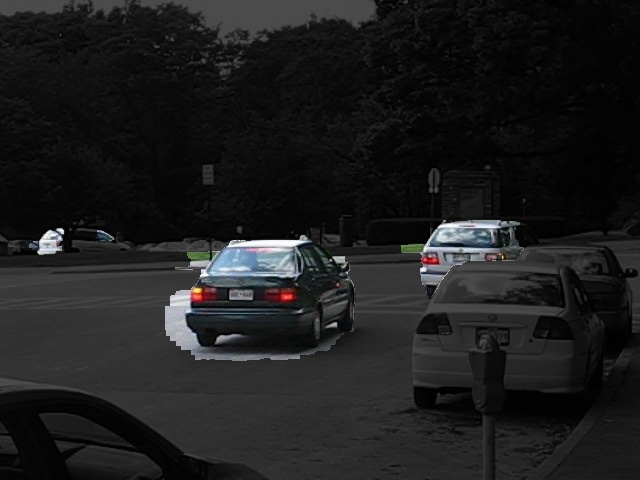
\includegraphics[width=0.18\textwidth]{ch5/moseg/c2_10.jpg}
  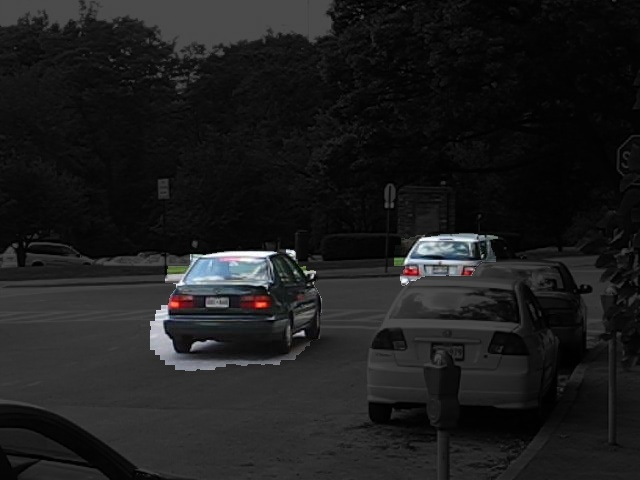
\includegraphics[width=0.18\textwidth]{ch5/moseg/c2_15.jpg}
  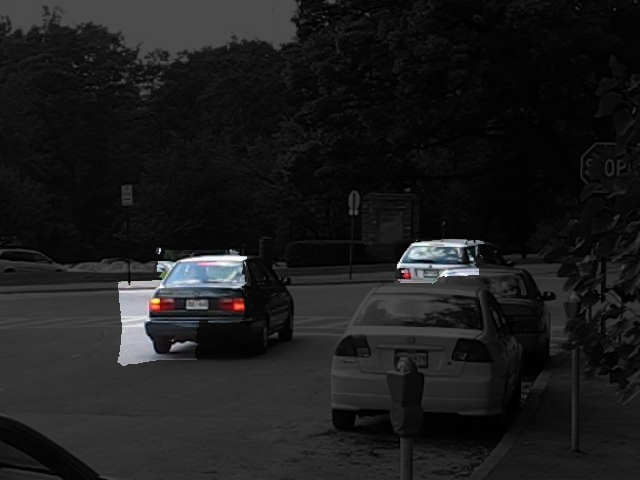
\includegraphics[width=0.18\textwidth]{ch5/moseg/c2_20.jpg}
  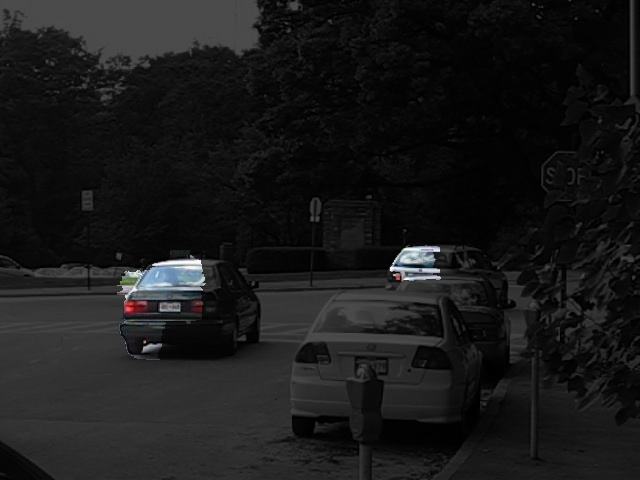
\includegraphics[width=0.18\textwidth]{ch5/moseg/c2_25.jpg} \\
(a) Cars2\\
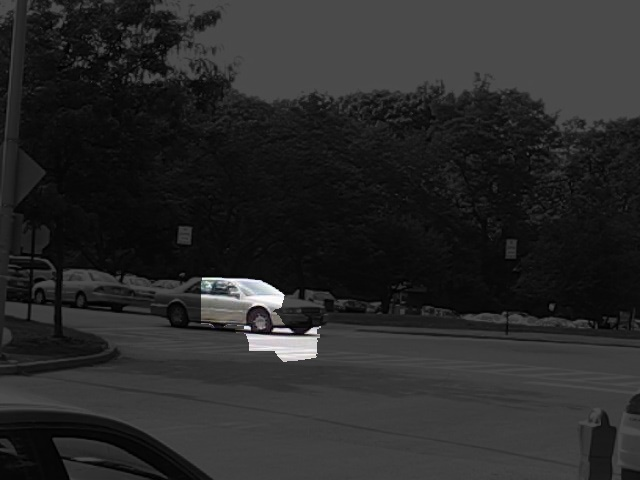
\includegraphics[width=0.18\textwidth]{ch5/moseg/c6_02.jpg}
  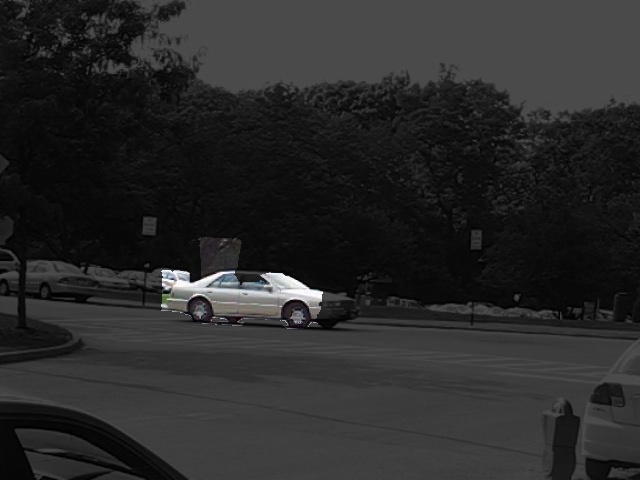
\includegraphics[width=0.18\textwidth]{ch5/moseg/c6_10.jpg}
  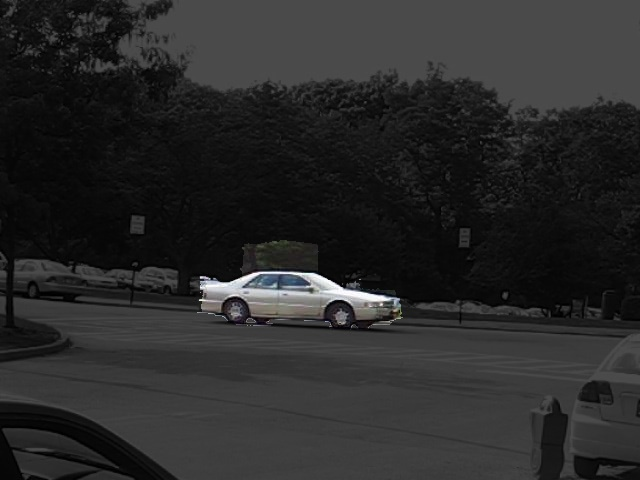
\includegraphics[width=0.18\textwidth]{ch5/moseg/c6_15.jpg}
  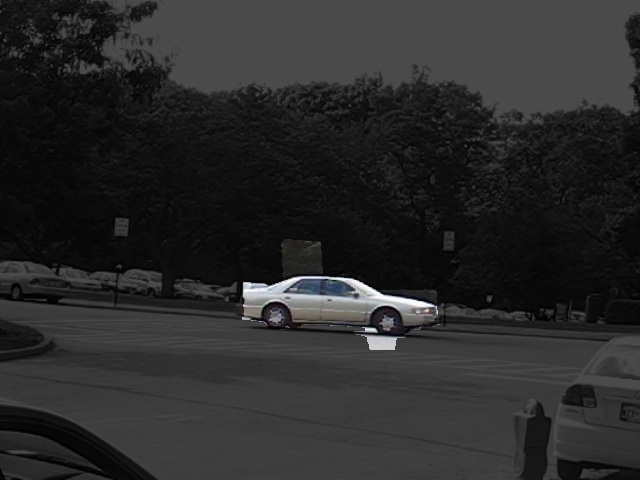
\includegraphics[width=0.18\textwidth]{ch5/moseg/c6_20.jpg}
  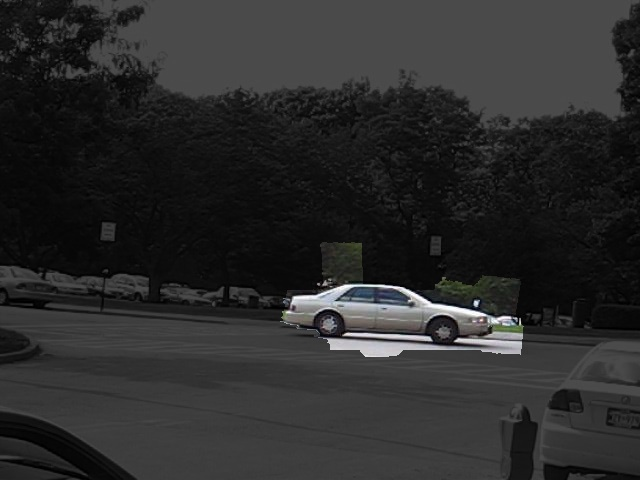
\includegraphics[width=0.18\textwidth]{ch5/moseg/c6_25.jpg} \\

(b) Cars6\\
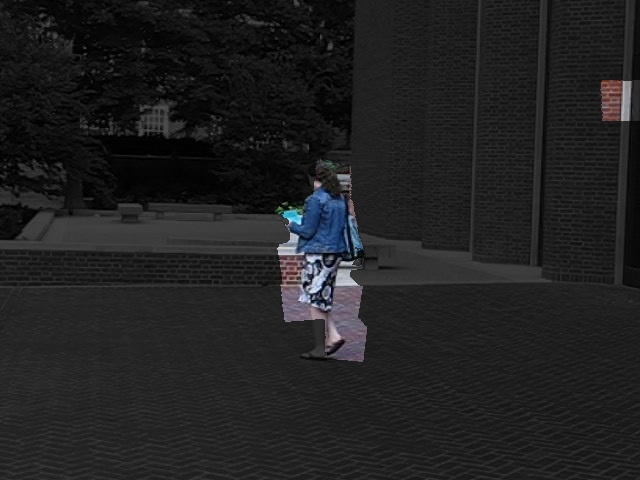
\includegraphics[width=0.18\textwidth]{ch5/moseg/p1_02.jpg}
  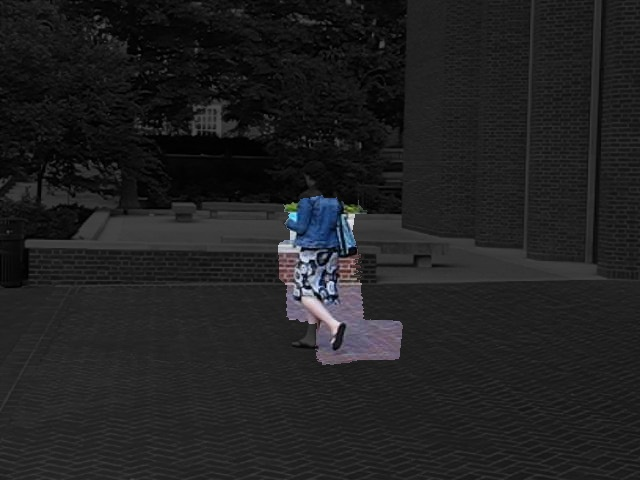
\includegraphics[width=0.18\textwidth]{ch5/moseg/p1_10.jpg}
  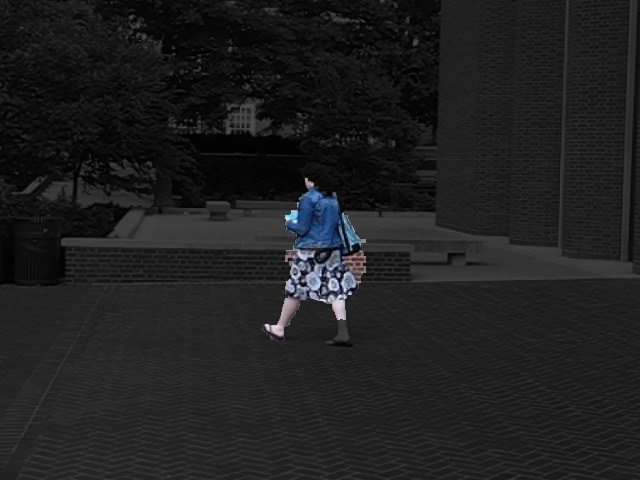
\includegraphics[width=0.18\textwidth]{ch5/moseg/p1_15.jpg}
  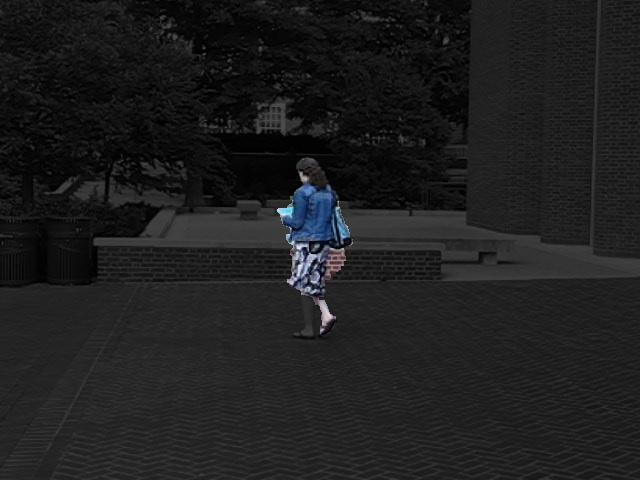
\includegraphics[width=0.18\textwidth]{ch5/moseg/p1_20.jpg}
  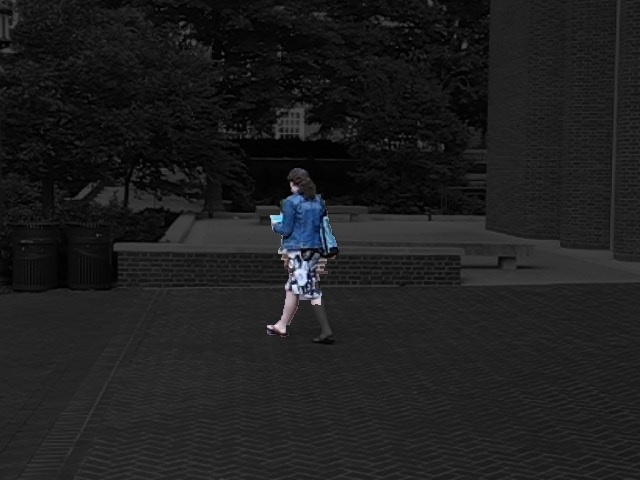
\includegraphics[width=0.18\textwidth]{ch5/moseg/p1_25.jpg} \\

(c) People1\\
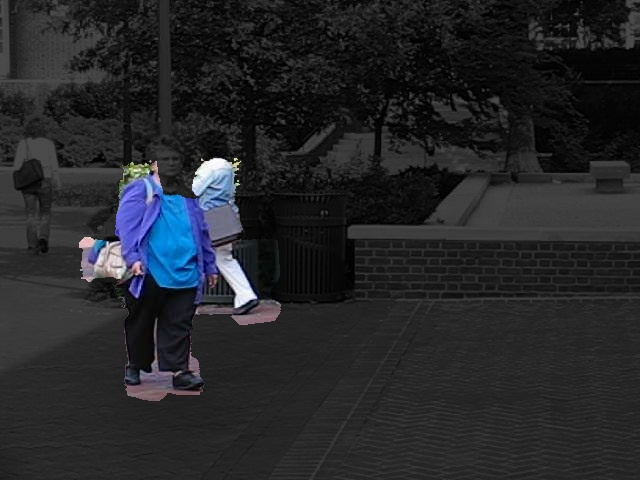
\includegraphics[width=0.18\textwidth]{ch5/moseg/p2_02.jpg}
  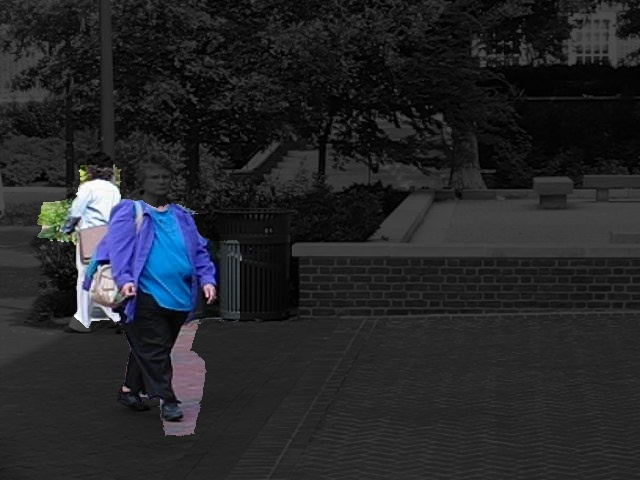
\includegraphics[width=0.18\textwidth]{ch5/moseg/p2_10.jpg}
  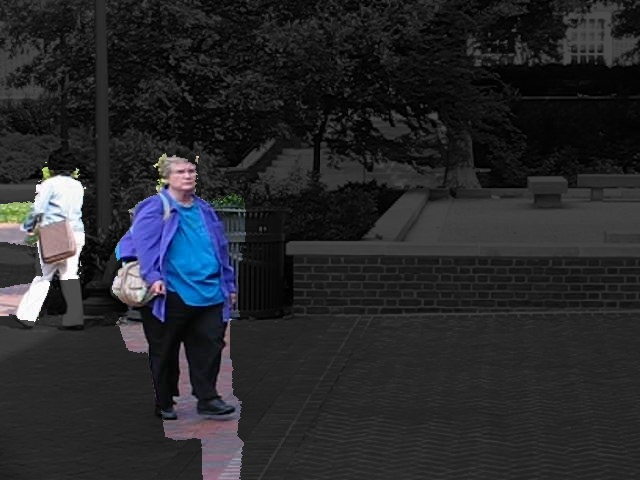
\includegraphics[width=0.18\textwidth]{ch5/moseg/p2_15.jpg}
  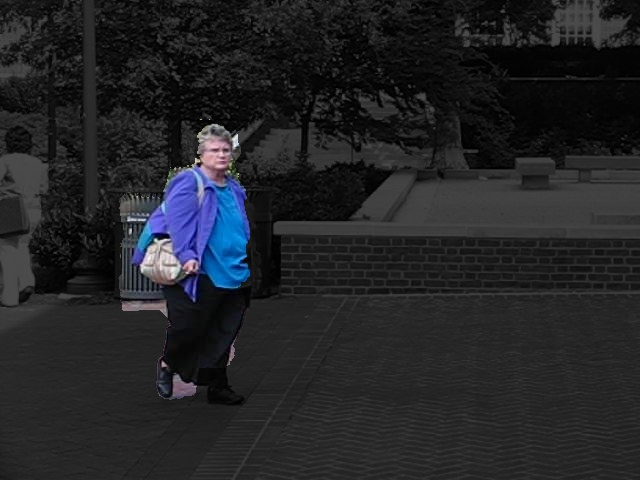
\includegraphics[width=0.18\textwidth]{ch5/moseg/p2_20.jpg}
  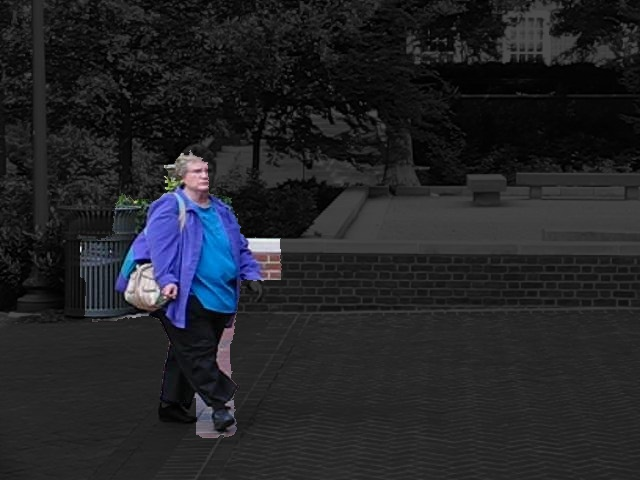
\includegraphics[width=0.18\textwidth]{ch5/moseg/p2_25.jpg} \\

(d) People2\\
\end{center}
\caption{本章算法在在Hopkins视频数据集\cite{HopKinsDataSet}中的部分结果}
\label{ch5:fig:MosegResults}       % Give a unique label
\end{figure}
将本文算法与文献~\inlinecite{5.8s,kwak2011Generalized}中的算法进行了比较,部分结果如图~\ref{ch5:fig:comparison}所示。图~\ref{ch5:fig:comparison}(a)中分别为Hopkins视频数据库中Cars1视频的第6帧, Cars3 视频的第11帧,Cars8视频的第16帧, People1视频的第19帧和Peopel2视频的第16帧。 图~\ref{ch5:fig:comparison}(b)所示为图~\ref{ch5:fig:comparison}(a)中视频帧的正确前景结果, 图~\ref{ch5:fig:comparison}(c)所示为文献~\inlinecite{kwak2011Generalized}算法的结果, 图~\ref{ch5:fig:comparison}(d)所示为文献~\inlinecite{5.8s}算法结果,  图~\ref{ch5:fig:comparison}(e)所示为本章算法结果。
\begin{figure}[ht]
  \centering
  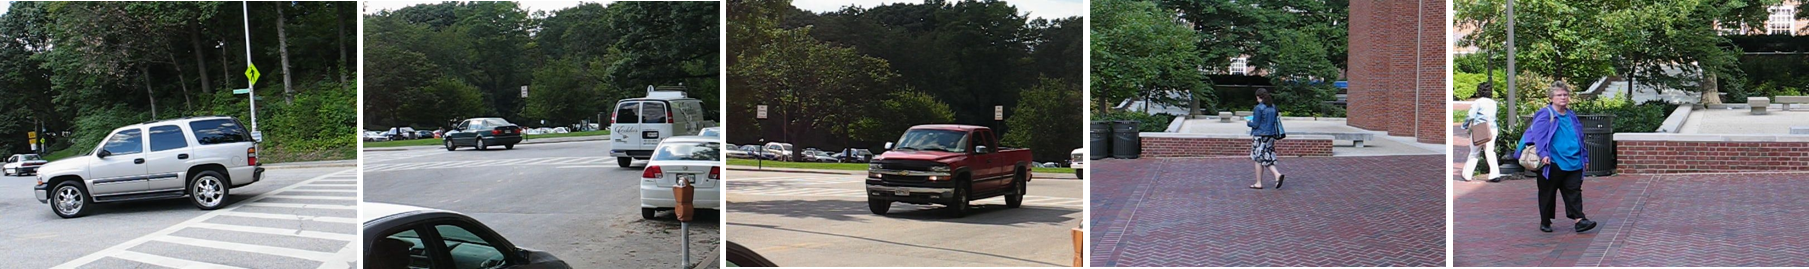
\includegraphics[width=0.9\textwidth]{ch5/fig5a.png}\\
  (a) 输入图像\\
   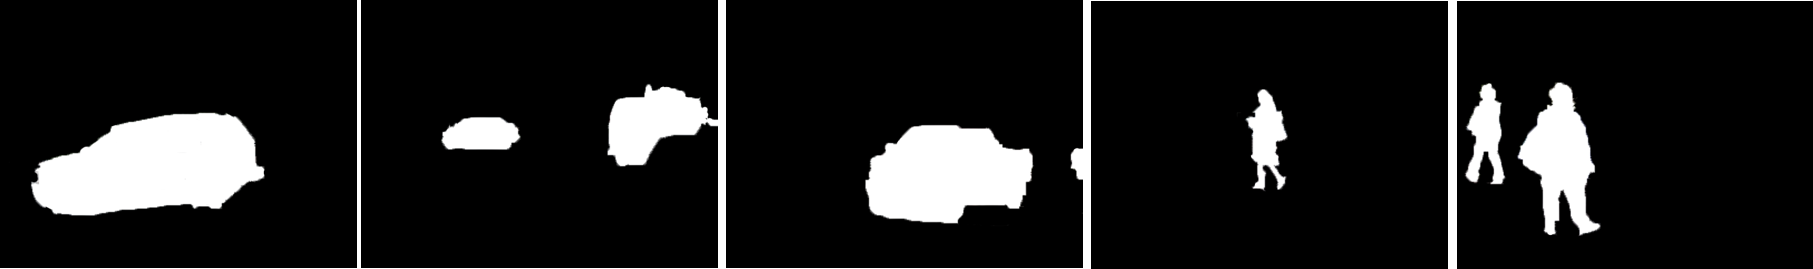
\includegraphics[width=0.9\textwidth]{ch5/fig5b.png}\\
   (b) 前景正确结果\\
   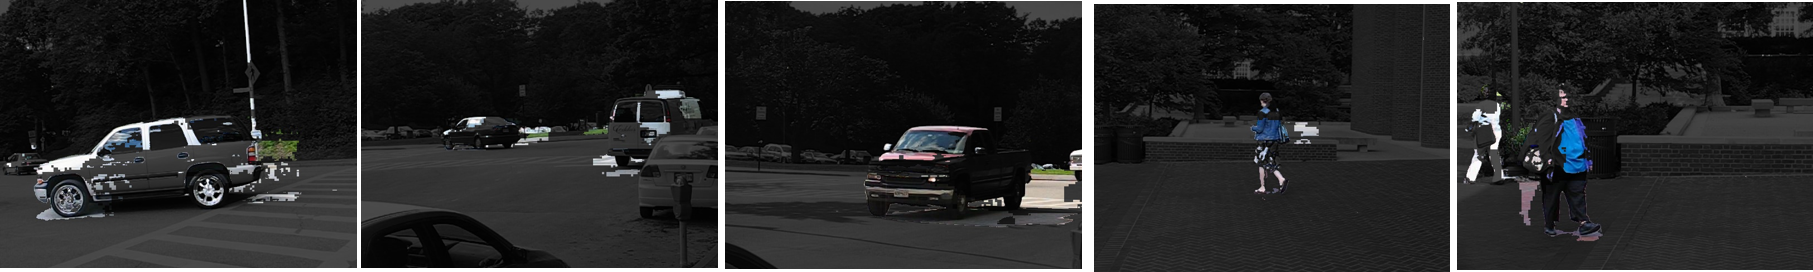
\includegraphics[width=0.9\textwidth]{ch5/fig5c.png}\\
   (c) 文献~\inlinecite{kwak2011Generalized}算法处理结果\\
   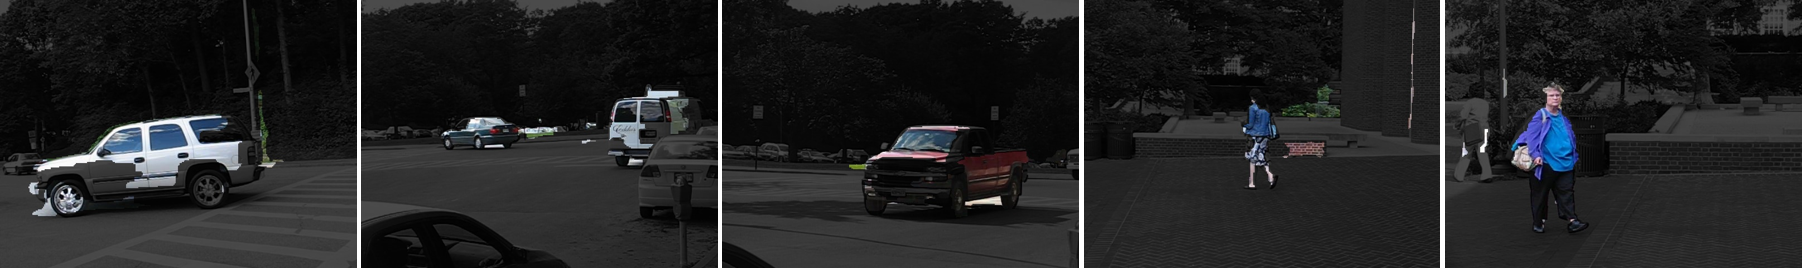
\includegraphics[width=0.9\textwidth]{ch5/fig5d.png}\\
   (c) 文献~\inlinecite{5.8s}算法处理结果\\
   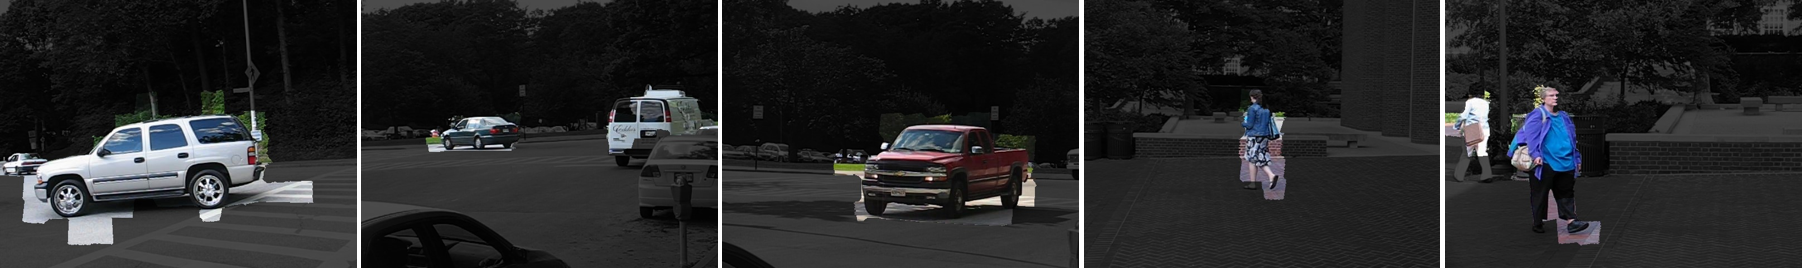
\includegraphics[width=0.9\textwidth]{ch5/fig5e.png}\\
   (c) 本章算法处理结果\\
  \caption{算法前景检测结果及比较}\label{ch5:fig:comparison}
\end{figure}


 本章采用通用的前景准确度指标,精度P, 召回率R和F值(F-Score, F)来量化评价算法的前景检测准确度。 本文算法与同类实时算法~\cite{5.8s}的部分结果如表~\ref{ch5:tab:comparison}所示。

\begin{table}[htb]

% table caption is above the table
\caption{算法准确度比较,最好的结果用粗体表示}
\label{ch5:tab:comparison}       % Give a unique label
% For LaTeX tables use
\centering
\begin{tabular}{ccccccc} \toprule[1.5pt]
\multicolumn{1}{c}{\multirow {2}{*}{}}&\multicolumn{3}{c}{本章算法}& \multicolumn{3}{c}{\inlinecite{5.8s}算法}\\
\cline{2-7}
\multicolumn{1}{c}{}&\multicolumn{1}{c}{P}&\multicolumn{1}{c}{R}&\multicolumn{1}{c}{F}&\multicolumn{1}{c}{P}&\multicolumn{1}{c}{R}&\multicolumn{1}{c}{F}\\
\hline

\multicolumn{1}{c}{cars1}&\multicolumn{1}{c}{\textbf{0.653}}&\multicolumn{1}{c}{\textbf{0.979}}&\multicolumn{1}{c}{\textbf{0.783}}&\multicolumn{1}{c}{0.640}&\multicolumn{1}{c}{0.336}&\multicolumn{1}{c}{0.441}\\
\multicolumn{1}{c}{cars2}&\multicolumn{1}{c}{\textbf{0.727}}&\multicolumn{1}{c}{\textbf{0.706}}&\multicolumn{1}{c}{\textbf{0.716}}&\multicolumn{1}{c}{0.399}&\multicolumn{1}{c}{0.908}&\multicolumn{1}{c}{0.789}\\
\multicolumn{1}{c}{cars3}&\multicolumn{1}{c}{\textbf{0.742}}&\multicolumn{1}{c}{\textbf{0.877}}&\multicolumn{1}{c}{\textbf{0.804}}&\multicolumn{1}{c}{0.640}&\multicolumn{1}{c}{0.956}&\multicolumn{1}{c}{0.882}\\
\multicolumn{1}{c}{cars4}&\multicolumn{1}{c}{\textbf{0.694}}&\multicolumn{1}{c}{\textbf{0.627}}&\multicolumn{1}{c}{\textbf{0.658}}&\multicolumn{1}{c}{0.676}&\multicolumn{1}{c}{0.917}&\multicolumn{1}{c}{0.895}\\
\multicolumn{1}{c}{cars5}&\multicolumn{1}{c}{{0.686}}&\multicolumn{1}{c}{\textbf{0.720}}&\multicolumn{1}{c}{0.845}&\multicolumn{1}{c}{\textbf{0.703}}&\multicolumn{1}{c}{\textbf{0.724}}&\multicolumn{1}{c}{\textbf{0.874}}\\
\multicolumn{1}{c}{cars6}&\multicolumn{1}{c}{0.620}&\multicolumn{1}{c}{\textbf{0.682}}&\multicolumn{1}{c}{\textbf{0.650}}&\multicolumn{1}{c}{\textbf{0.726}}&\multicolumn{1}{c}{0.726}&\multicolumn{1}{c}{0.903}\\
\multicolumn{1}{c}{cars7}&\multicolumn{1}{c}{\textbf{0.687}}&\multicolumn{1}{c}{\textbf{0.957}}&\multicolumn{1}{c}{\textbf{0.800}}&\multicolumn{1}{c}{{0.657}}&\multicolumn{1}{c}{0.950}&\multicolumn{1}{c}{\textbf{0.869}}\\
\multicolumn{1}{c}{cars8}&\multicolumn{1}{c}{\textbf{0.692}}&\multicolumn{1}{c}{\textbf{0.975}}&\multicolumn{1}{c}{\textbf{0.810}}&\multicolumn{1}{c}{0.653}&\multicolumn{1}{c}{0.944}&\multicolumn{1}{c}{0.826}\\
\multicolumn{1}{c}{people1}&\multicolumn{1}{c}{{0.486}}&\multicolumn{1}{c}{\textbf{0.861}}&\multicolumn{1}{c}{\textbf{0.621}}&\multicolumn{1}{c}{\textbf{0.887}}&\multicolumn{1}{c}{0.816}&\multicolumn{1}{c}{0.866}\\
\multicolumn{1}{c}{people2}&\multicolumn{1}{c}{\textbf{0.732}}&\multicolumn{1}{c}{\textbf{0.866}}&\multicolumn{1}{c}{\textbf{0.794}}&\multicolumn{1}{c}{0.834}&\multicolumn{1}{c}{0.602}&\multicolumn{1}{c}{0.699}\\
\hline
\multicolumn{1}{c}{平均}&\multicolumn{1}{c}{\textbf{0.680}}&\multicolumn{1}{c}{\textbf{0.829}}&\multicolumn{1}{c}{\textbf{0.747}}&\multicolumn{1}{c}{0.664}&\multicolumn{1}{c}{0.300}&\multicolumn{1}{c}{0.414}\\
\bottomrule[1.5pt]

\end{tabular}

\end{table}

 为了实现实时处理, 本文使用了基于超像素的快速区域分割预处理算法,从图~\ref{ch5:fig:comparison}和表~\ref{ch5:tab:comparison}中通过比较可以看出, 在大多数情况下本文算法能有效的检测视频中的前景部分, 而文献\inlinecite{5.8s}的算法在很多情况下得不到满意的结果。\par
本文算法处理大小为$640 \times 480$像素的视频的平均速度约为28帧/秒, 可以满足实时处理的需要; 文献~\inlinecite{5.8s}算法处理同样大小的视频速度要快于本文算法, 约为45帧/秒, 但其前景检测准确度较低, 在相机运动幅度较大时算法无法有效工作。 综合考虑前景检测准确度和处理速度,本文算法更适合实时的实际应用。


\section{本章小结}
\label{ch5:sec:conclusions}
随着移动设备软硬件的不断升级,目前智能手机、平板电脑等移动计算平台的计算能力越来越强,已经达到甚至超越了传统桌面个人电脑的计算能力。这使得在移动计算平台上可以实现一些计算密集型任务,例如实时的图像和视频处理任务。视频背景减除技术应用范围广,不仅常用于视频编辑等离线应用,也经常用于实时监控等实时任务。当拍摄视频的摄像机为移动相机时,实现实时的视频背景减除是较困难的一项任务。准确提取移动相机拍摄视频中的前景对象本身就是一项困难的工作,其中包含估算相机运动,背景建模等计算密集型步骤,而在此基础上实现实时处理则更加困难。目前能实时完成移动相机视频背景减除计算的算法较少。为了实现实时处理,文献~\inlinecite{5.8s}对输入图像进行了分块处理,为每个分块建立一个双模式的高斯模型。而在处理相机运动时,仅计算每个分块角点的稀疏光流,并估算全局单应性矩阵。虽然文献~\inlinecite{5.8s}的速度非常快,但是由于背景模型的精度过低,以及相机运动补偿算法过于简单,使得该算法的前景检测准确度较差,无法处理稍微复杂一些的场景或较快移动的而相机等情况。\par
为了在保证前景检测精度的前提下实现移动相机拍摄视频的实时背景减除,本章提出了一种简单有效的算法。 不同于已有的算法, 本章算法不需要计算稠密光流或点轨迹, 也不需要建立并更新背景模型。 根据背景的连续性特点, 通过基于超像素的区域增长算法进行预处理, 先将较为明显的背景去除。在自然图像中,背景部分具有较明显的连续性,特别是在室外场景拍摄的视频中,这种连续性尤为明显,例如天空、地面、墙面、草地、树林等。在通过区域增长算法对图像进行区域分割的过程中,背景区域由于连续性明显,将会较为容易的被合并到一个大区域中,而前景区域相对背景区域则会显得面积更小。利用这一特点,可以快速的得到可能是前景的区域。随后根据基于相对光流和分块估计的算法利用匹配特征点估算相机的运动,对可能的前景超像素进行验证, 比较其光流和相机运动的一致性,获得最终的前景结果。在移动相机拍摄视频中,区分前景和背景的一个重要线索是对象的运动情况,由于背景部分是相对静止的,因此背景区域像素的光流应该由相机的运动决定,而前景部分像素的光流则由前景本身的运动决定。因此本章算法通过判别光流和相机运动之间的距离是否在允许的门限之内进一步判断经过预处理得到的疑似前景对象是否确实属于前景。本章算法简单直接, 借助GPU能实现实时处理。大量的实验证明了其有效性, 特别是室外拍摄的背景连续性较强的视频 。相比于同类实时算法, 本文算法的前景检测准确率更高; 而与基于稠密光流或点轨迹的算法相比, 本文算法的处理速度有明显优势。\par
因为本文算法是建立在前景占视频中较小的部分的假设的, 因此无法处理视频中前景占据主要部分,或者匹配的特征点集中在前景的情况。 此外, 本文算法不适合处理背景连续性较差的视频, 如室内拍摄视频或包含复杂背景的视频。 针对这些视频, 本章的区域分割算法可能会失效。 在未来的工作中, 我们将考虑解决上述问题,并在保持算法实时性的前提下 进一步提高算法的前景检测准确度。
